% 
%	Jan Kechel
%	
%
\documentclass[landscape]{slides}
\usepackage{color,german}
\usepackage{graphics}
\usepackage[latin1]{inputenc}
%
\begin{document}
%
\title{TeamFound\\Infrastrukturen zur Open Source Softwareentwicklung\\Technische Universit"at Berlin}
\author{A. Bachmann, J. Heese, J. Kechel, M. Klink}
\date{WS 2005/2006}

%
\maketitle%
%
%%
\begin{slide}{Gliederung}

\textbf{1. Einf"uhrung}\\
Idee, Zielsetzung, Architektur-"Uberblick, Interface

\textbf{2. Server}\\
Architektur, Lucene, Datenstrukturen, Interner Ablauf 

\textbf{3. Organisation / Verlauf}\\
Kommunikation, Treffen, Ablauf

\textbf{4. Implementation Clients}\\
Web-Client, Firefox Toolbar, IE Toolbar

\textbf{5. Pr"asentation}
\end{slide}
%
%
%
%
\begin{slide}{1.1 Was ist TeamFound?}\\

TeamFound ist...

\begin{itemize}
\item eine Suchmaschine
\item nicht mit einem eigenen Crawler ausger"ustet
\item nicht auf einem lokalen Computer sondern "uber einen Webserver erreichbar
\item daher von beliebig vielen Menschen benutzbar
\end{itemize}

\end{slide}
%
\begin{slide}{1.2 Was bringt TeamFound?}\\

Einfacher UseCase:

\begin{itemize}
\item Alice will ihre E-Mails verschl"usseln und sucht nach geeigneter Software
\item Alice findet GnuPG und speichert ihr Suchergebnis in TeamFound
\item Bob sucht ebenfalls nach einer solchen L"osung
\item Bob findet sofort den Eintrag von Alice im TeamFound
\end{itemize}
\end{slide}
%
\begin{slide}{1.2 Oder anders}\\

Denkbar auch f"ur:

\begin{itemize}
\item Alle m"oglichen Teams mit Rechercheaufwand (Open-Source, Softwareentwicklung, ...)
\item Studenten \& Recherche f"ur Vorlesungen
\item Lose Gruppen mit bestimmten Themen (Angeln, Ski-Fahren,...)
\end{itemize}
\end{slide}

\begin{slide}{1.4 Wie funktioniert TeamFound?}\\

\begin{itemize}
\item TeamFound bietet Integrationen f"ur Internet-Explorer und Firefox
\item TeamFound zeigt eigene + Google-Ergebnisse
\item TeamFound kann auch wie andere Suchmaschinen "uber eine Webseite benutzt werden
\item Neue Seiten k"onnen mit wenigen Klicks hinzugef"ugt werden
\end{itemize}
\end{slide}

%mit zu 1. ?
\begin{slide}{1.x Request/Response }\\
\begin{itemize}
\item Anfrage-Parameter werden in Form von HTTP GET Variablen "ubertragen
\item Antworten vom Server
\begin{itemize}
\item HTML-Seite: die direkt im Browser angezeigt wird
\item XML-File: wird von der Toolbar interpretiert
\end{itemize}	
\end{itemize}
\end{slide}
%
\begin{slide}{1.x Beispiel Request}\\
\begin{verbatim}
http://62.75.187.241:8080/tf/tf?keyword=teamfound
&want=xml&version=2&command=search&category=1
\end{verbatim}
\end{slide}
\begin{slide}{1.x Beispiel Response }\\
\begin{verbatim}
<response>
	.
	.
	<search>	
		<result>
			<found>
				<url>http://teamfound.berlios.de</url>
				<title>TeamFound - share your search results</title>
				<incategory>0</incategory>
			</found>
		</result>
	</search>
</response>
\end{verbatim}
\end{slide}
%
%
%
\begin{slide}{2 Server}\\
\end{slide}
%
\begin{slide}{2.1 Architektur des Servers}\\
\begin{center}
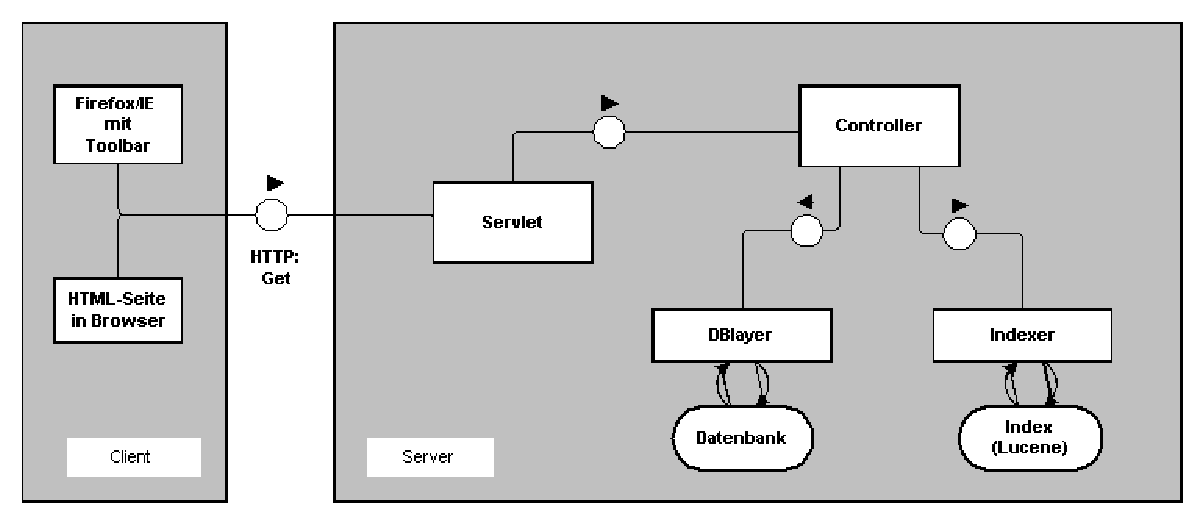
\includegraphics{bilder/aufbau2.eps}
\end{center}
\end{slide}
%
\begin{slide}{2.2 Lucene Index}
\begin{itemize}
\item Wichtige Komponenten von Apache Lucene:
\begin{itemize}
\item Document und Field
\item Analyzer
\item Query
\end{itemize}
\end{itemize}
\end{slide}
%
\begin{slide}{2.3 Datenstrukturen}\\
\begin{center}
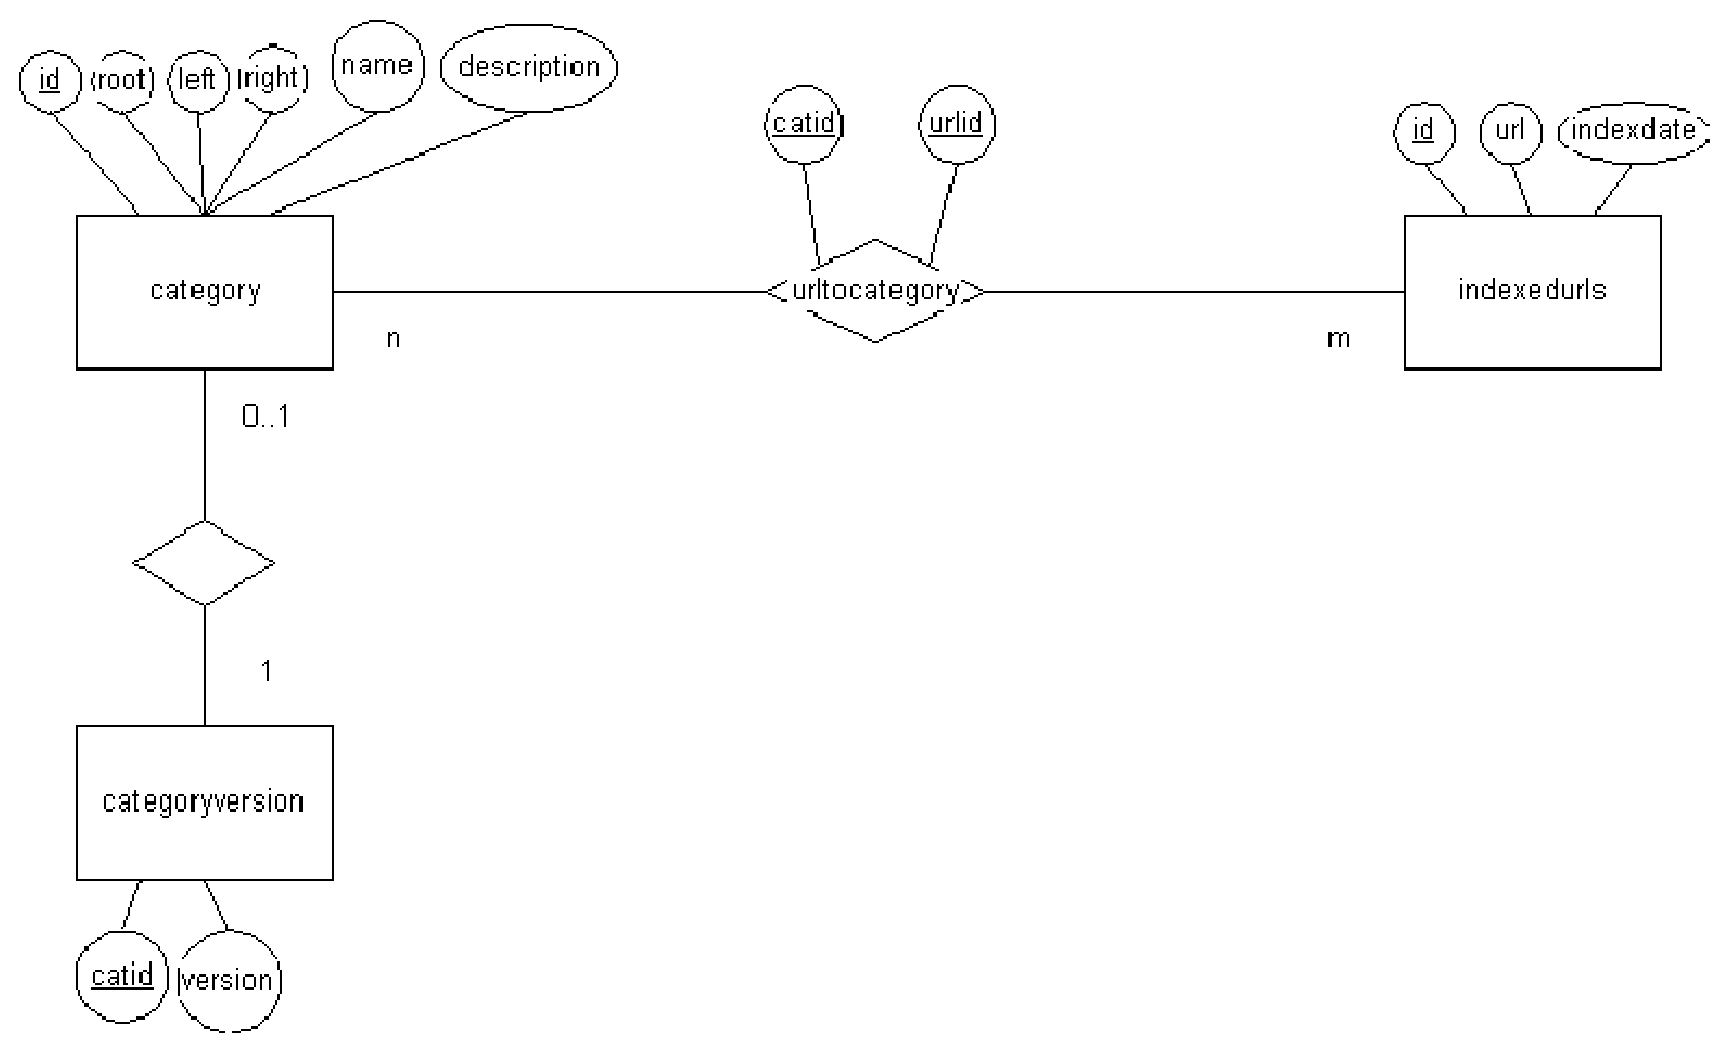
\includegraphics{bilder/db.eps}
\end{center}
\end{slide}
%	
\begin{slide}
\begin{center}
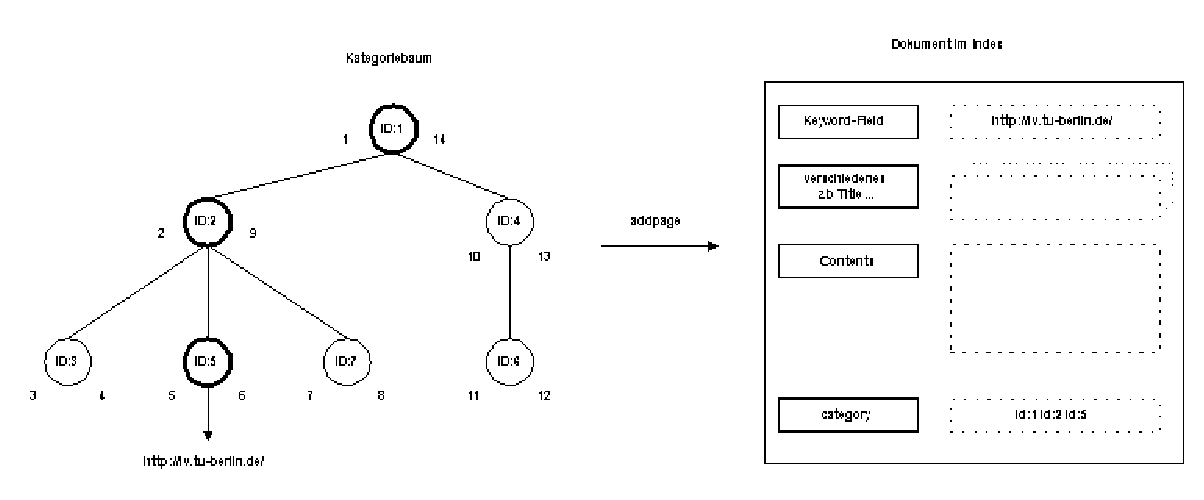
\includegraphics{bilder/katstruktur}
\end{center}
\end{slide}
%
\begin{slide}{2.5 Hinzuf"ugen einer Seite}
\begin{itemize}
\item Url auf vorhandensein "Uberpr"ufen :
\begin{enumerate}
\item Url existiert nicht: Download, Indexeintrag, Datenbankeintrag  
\item Url existiert : Dokument auslesen, Dokument l"oschen, 
aktualisiertes Dokument erstellen und hinzuf"ugen, Datenbankeintrag
\end{enumerate}
\item Response erstellen
\end{itemize}
\end{slide}
%
\begin{slide}{2.6 Suchen einer Seite}
\begin{itemize}
\item Query erstellen
\item Anfrage an Index 
\item Response erstellen
\end{itemize}
\end{slide}
%
%
%
\begin{slide}{3. Organisation}\\
\end{slide}
%
%
%
\begin{slide}{3.1 Kommunikation}
\begin{itemize}
\item MediaWiki f"ur Entwicklungs-Arbeit (Standards, Interfaces, Realisierungen) \texttt{http://wiki.jonasheese.de/index.php/TeamFound}

\item TeamFound - Mailingliste \texttt{teamfound-development@lists.berlios.de}

\item OSSI - Mailingliste \texttt{ossi@insel.cs.tu-berlin.de} 

\item Chat - QuakeNet \#teamfound 
\end{itemize}


\end{slide}
%
%
%
\begin{slide}{3.2 Source-Code Verwaltung}
\begin{itemize}
\item BerliOS Developer
\item Project page  \texttt{https://developer.berlios.de/projects/teamfound}
\item SVN server \texttt{svn.berlios.de}
\item Web server \texttt{http://teamfound.berlios.de}
\end{itemize}
\end{slide}
%
%
%
\begin{slide}{3.3 Teilprojekte}
\begin{itemize}
\item Milestones
\item Toolbar Firefox, Toolbar Internet Explorer, Web-Client
\item Server
\item Interface-Spezifikation
\item Pr�sentation
\item Kategorien
\end{itemize}
\end{slide}
%
%
%
\begin{slide}{3.4 Milestone 1}
\begin{enumerate}
\item Lauff�hige Versionen der Toolbars und des Servers
\item �ber Toolbar einzelne HTML-Seiten hinzuf�gen
\item Server soll diese HTML-Seiten indizieren und durchsuchbar machen
\item �ber Toolbar soll der Server zum durchsuchen der indizierten Seiten nach Schl�sselw�rtern gebracht werden und ein Liste der Links als Web-Seite zur�ckliefern 
\end{enumerate}
\begin{verbatim}
[ Hinzufuegen-Button ] [<--   textfeld   -->] [ Suchen-Button ]
\end{verbatim}
\end{slide}
%
%
%
\begin{slide}{3.5 Milestone 2}
\begin{itemize}
\item Kategorien-System
\item Konfigurations-Dialog in Toolbars f�r Server-Adresse
\item Zus�tzlich das Suchergebnis von google mit den gleichen Key-W�rtern anzeigen
\item Interface-Version Milestone 2 implementieren
\item XML oder HTML als Antwort von Server anfordern 
\end{itemize}
\end{slide}
%
%
%
\begin{slide}{3.6 Milestone 3}
\begin{itemize}
\item User-Management
\item Rating Mechanismen 
\end{itemize}
\end{slide}
%
%
%
\begin{slide}{3.7 Ideen f"ur zuk"unftige Versionen}
\begin{itemize}
\item Mehrere Server in Toolbar einstellbar
\item Mehrere Server �ber Toolbar in einem rutsch durchsuchen und die Ergebnisse kombinieren
\item Web-Interface f�r Server (und Server-Administration)
\item mehrere Sprachen unterst�tzen
\end{itemize}
\end{slide}
%

\begin{slide}{4. Client Implementationen}
\end{slide}
%
\begin{slide}{4.1 Web-Client}\\
\\

\includegraphics{webclient.eps}
\begin{verbatim}
javascript:location.href='http://serverurl/addpage.pl?
url='+encodeURIComponent(location.href)

<form action="serverurl">
	search: <input type="text" name="keyword">
	<input type="hidden" name="want" value="html">
	<input type="hidden" name="version" value="2">
	<input type="hidden" name="command" value="search">
	<input type="submit">
</form>
\end{verbatim}

\end{slide}
%
\begin{slide}{4.2 Firefox Toolbar}\\
\\
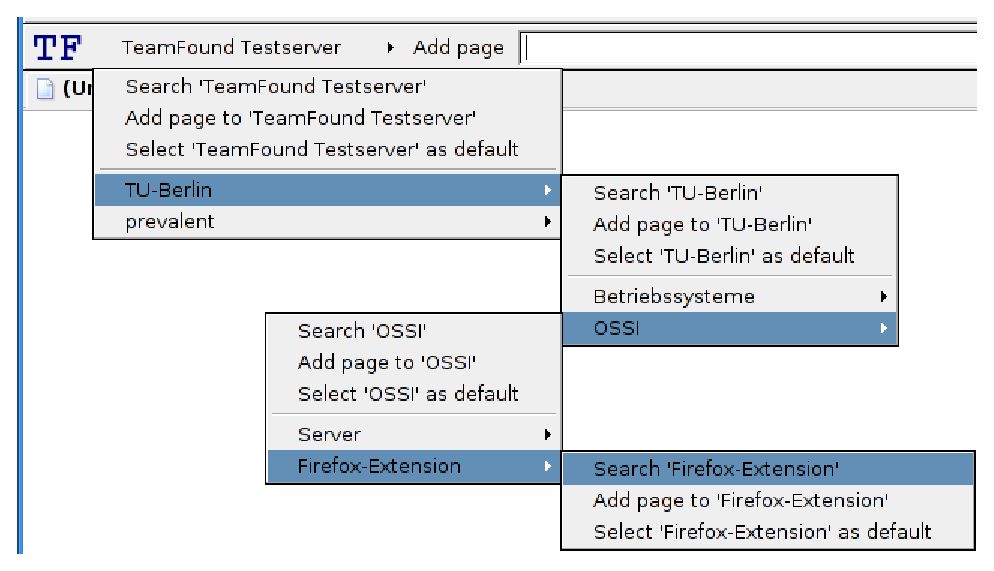
\includegraphics{ffextension-kategorien}
\end{slide}
%
%
\begin{slide}{4.3 Firefox Toolbar}\\
\\
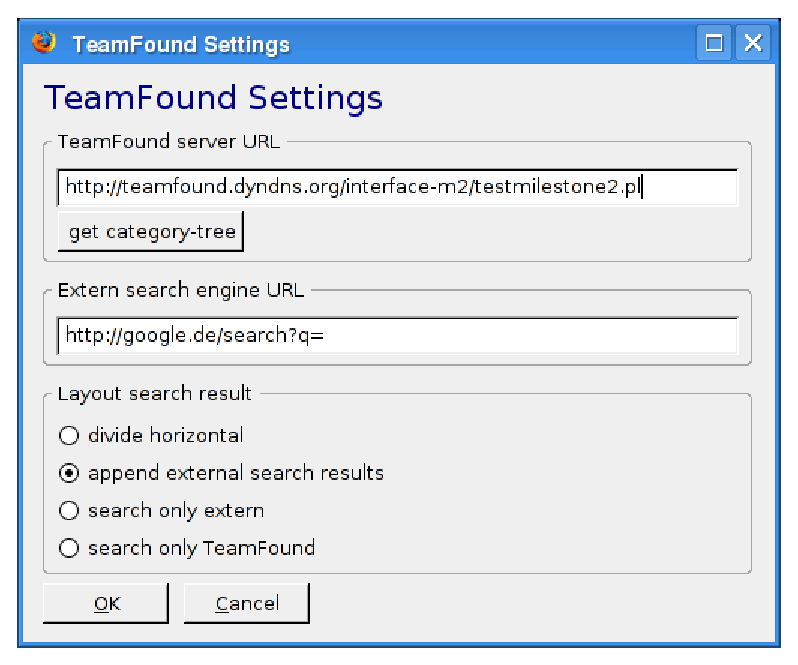
\includegraphics{ffextension-settings}
\end{slide}
%
%
%
\begin{slide}{4.3 Internet Explorer Toolbar}\\
IE Toolbar ..
\end{slide}
%%
%%
%
\begin{slide}{5.1 Pr"asentation}
\end{slide}
%
%
%
%
\begin{slide}{}
The End
\end{slide}
%%%%%%%%%%%%%%%%%%%%%%%
\end{document}
